% Chapter 1 — Meet KayanOS through your own work. Under review.
\chapter{Start with KayanOS}
\label{ch:intro}

\section{What is KayanOS?}
\label{sec:intro-minute}

\textbf{KayanOS} brings employees, tasks, requests and files into one workspace. See who owns the work and its status, within your permissions.

\begin{table}[H]
\centering
\caption{What do you need?}
\label{tab:intro-minute}
\rcZebra
\begin{tabularx}{\linewidth}{R{3.2cm} Y Y}
\rcHeaderRow
\thh{You need} & \thh{Use} & \thh{You will see}\\
Track work & Tasks & Owner, due date, status\\
Organize people & HR & Employee, job, working time\\
Collect complete requests & Forms and requests & Request details and review flow\\
Find a document & Files and attachments & The document linked to the work\\
Review progress & Projects and dashboards & Status of recorded work\\
\end{tabularx}
\end{table}

Define responsibilities, enter correct data and keep status up to date.

\section{Example: Horizon}
\label{sec:intro-entity}

Our fictional example: Horizon Services Co. in Damascus and Aleppo. Sarah handles HR; Omar coordinates operations.

\textbf{Before:} an office-setup request is lost in chat. Who will do it, and when?

\begin{figure}[H]
\centering
\begin{tikzpicture}[node distance=0.4cm,stepBox/.append style={minimum width=6cm,text width=5.6cm,minimum height=0.7cm}]
  \node[stepBox] (s0) {Record the office\\request};
  \node[stepBox,below=of s0] (s1) {Assign Omar and set a\\due date};
  \node[stepBox,below=of s1] (s2) {Update status and\\attach the result};
  \node[stepBox,below=of s2] (s3) {Review the result with\\the manager};
  \draw[flowsTo] (s0) -- (s1);
  \draw[flowsTo] (s1) -- (s2);
  \draw[flowsTo] (s2) -- (s3);
\end{tikzpicture}
\rclegend
\caption{After: a clear request and a reviewable result}
\label{fig:intro-workday}
\end{figure}

The team performs these steps; automation needs setup.

\section{Where to start}

\begin{table}[H]
\centering
\caption{Start according to your responsibility}
\label{tab:intro-roles}
\rcZebra
\begin{tabularx}{\linewidth}{R{3.4cm} Y Y}
\rcHeaderRow
\thh{Your role at work} & \thh{What you want to achieve} & \thh{Where do you start?}\\
Business owner or manager & Choose the first work to organize. & This chapter, then a small example.\\
System setup administrator & Prepare the organization and team. & Chapter~\ref{ch:org-setup}.\\
HR officer & Organize employees, working hours, leaves and payroll. & Chapter~\ref{ch:hr}, after the team is set up.\\
Employee & Reach and follow their own work. & Sign in below; the organization exists.\\
\end{tabularx}
\end{table}

Start with two employees, two jobs and one shift. Check, then expand.

\section{First sign-in}
\label{sec:intro-app-map}

\textbf{You need:} the organization address and sign-in method from your administrator. Example: hzn.kayanos.app. To create an organization, see Chapter~\ref{ch:org-setup}.

\begin{enumerate}
  \item Open the address. Sign in using the email, phone or employee ID prepared for you.
  \item Check the organization name before entering data.
\end{enumerate}

\begin{figure}[H]
\centering
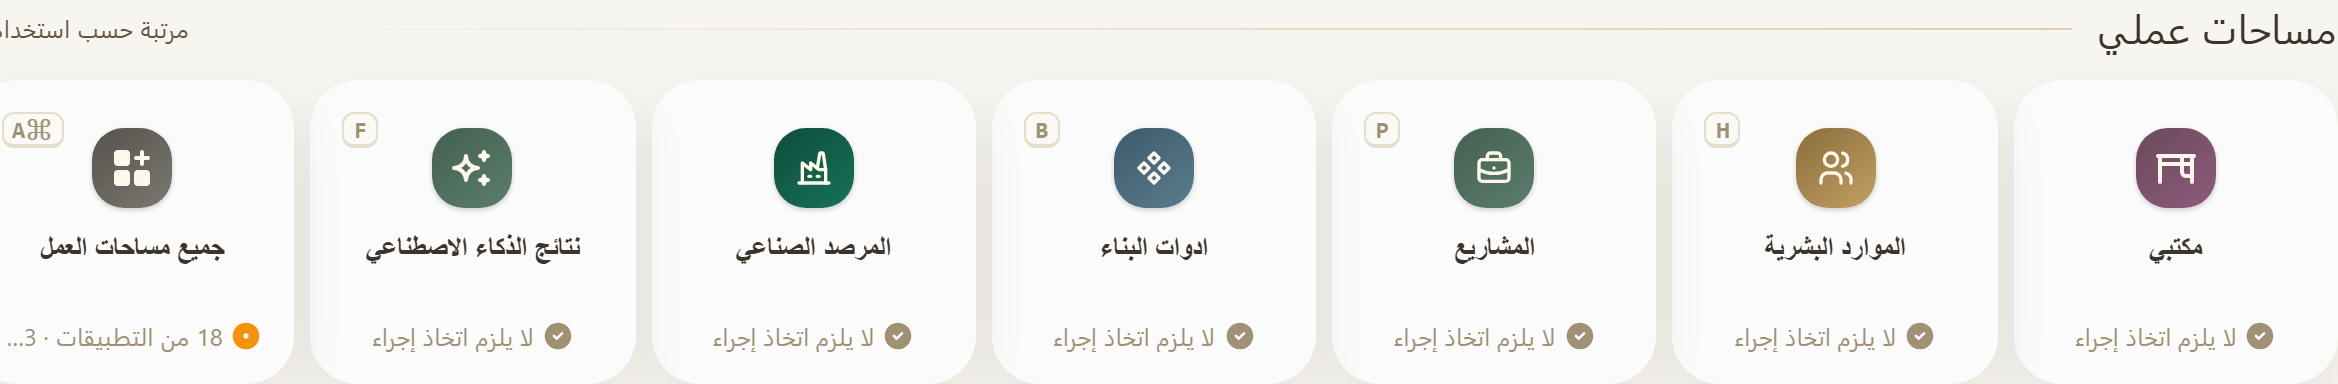
\includegraphics[width=0.95\linewidth]{figures/screens/ch01-workspaces-clear.png}
\caption{Open HR or All workspaces (Arabic interface)}
\label{fig:intro-home}
\end{figure}

\begin{figure}[H]
\centering
\begin{tikzpicture}[node distance=0.4cm,stepBox/.append style={minimum width=6cm,text width=5.6cm,minimum height=0.7cm}]
  \node[stepBox] (s0) {App launcher};
  \node[stepBox,below=of s0] (s1) {HR};
  \node[stepBox,below=of s1] (s2) {Members};
  \node[stepBox,below=of s2] (s3) {Employee name: details};
  \draw[flowsTo] (s0) -- (s1);
  \draw[flowsTo] (s1) -- (s2);
  \draw[flowsTo] (s2) -- (s3);
\end{tikzpicture}
\rclegend
\caption{Open a list, then one record}
\label{fig:intro-navigation}
\end{figure}

\begin{figure}[H]
\centering
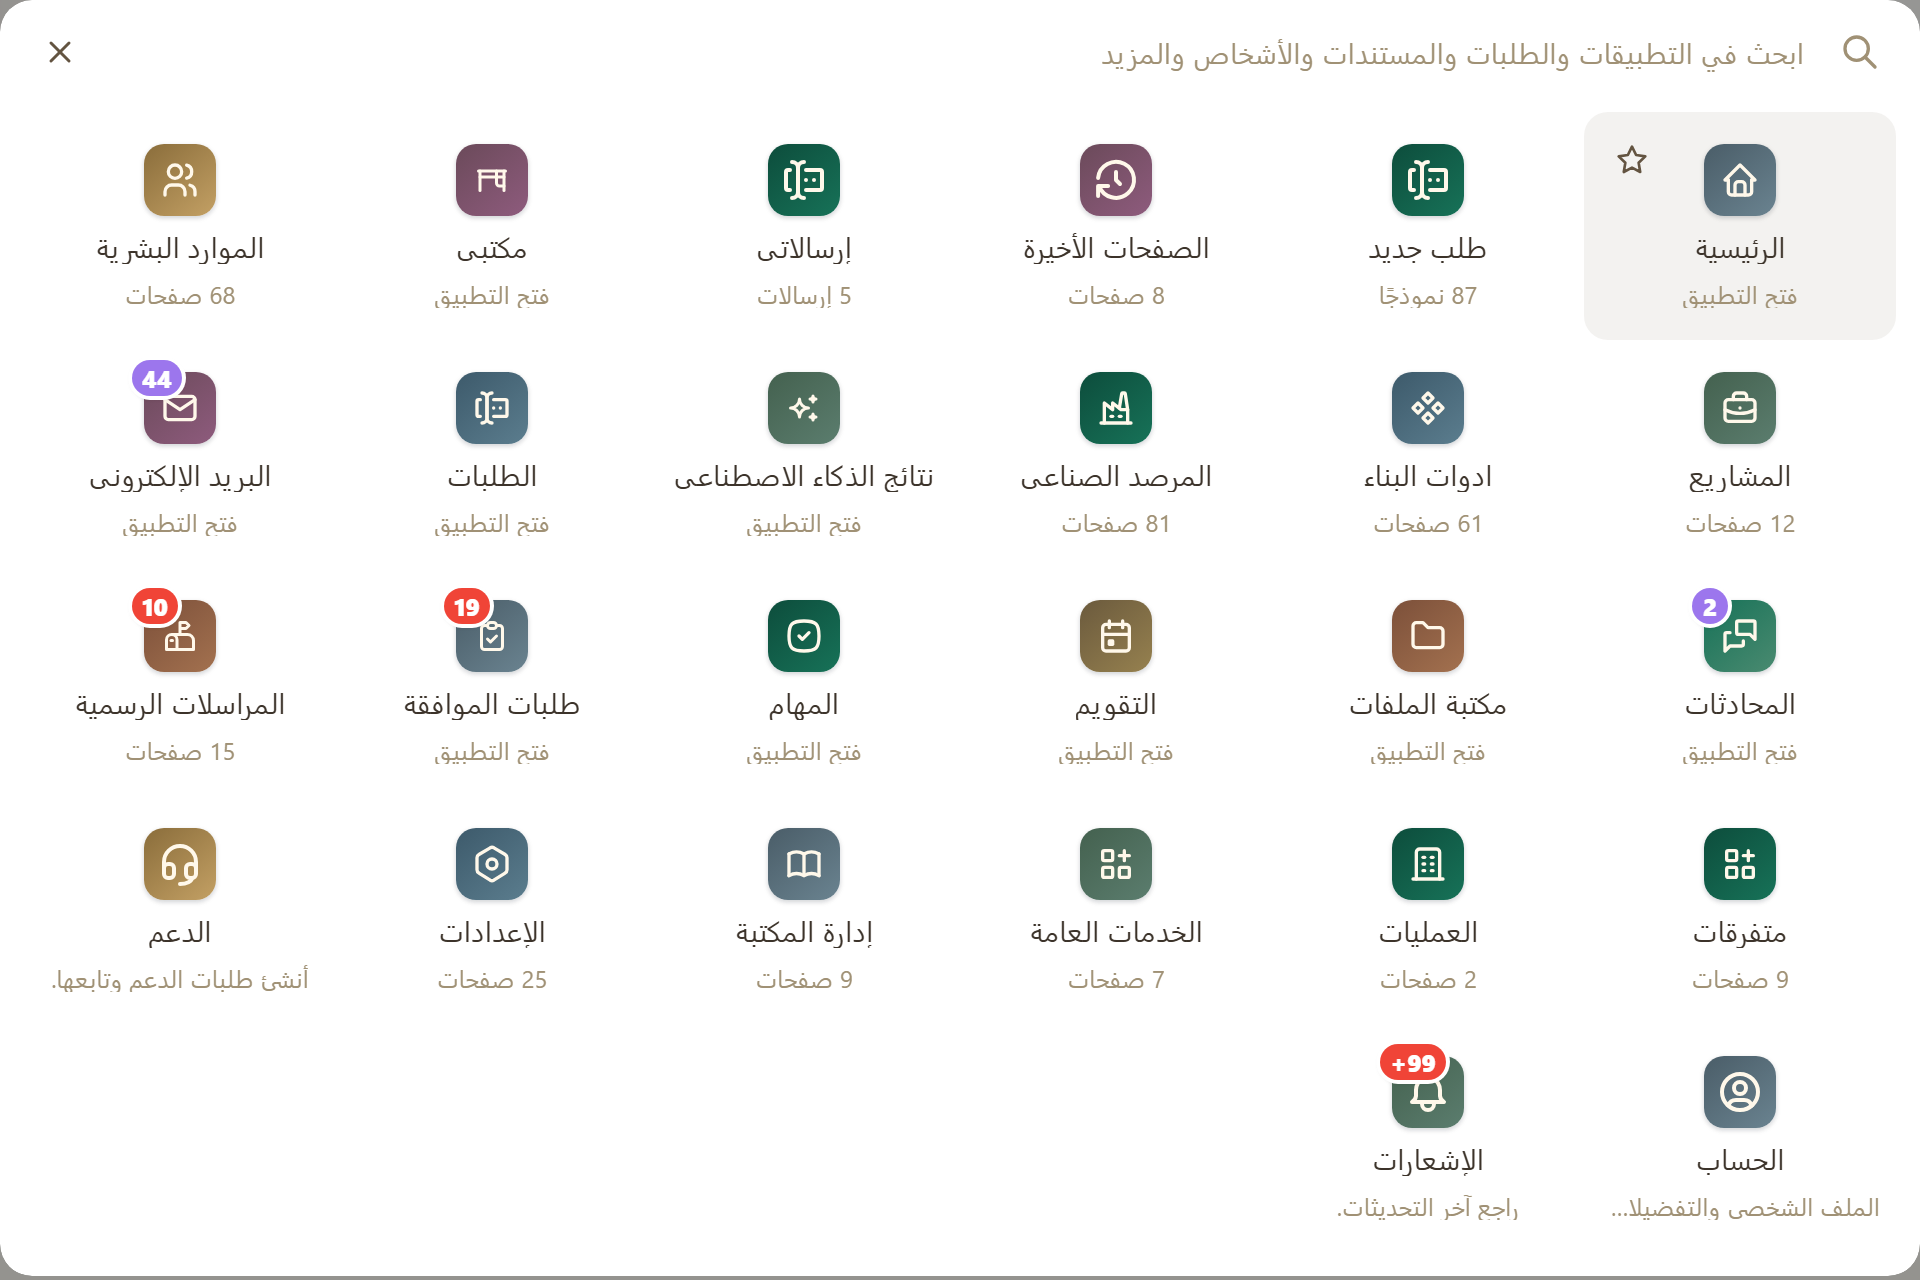
\includegraphics[width=0.95\linewidth]{figures/screens/ch01-apps-clear.png}
\caption{Choose an app (Arabic interface)}
\label{fig:intro-apps-directory}
\end{figure}

\textbf{Check:} open a member you can access. Return using the top navigation path. If an app or edit button is missing, ask the administrator to check permissions.

\section{Names to know}
\label{sec:intro-concepts}

\begin{table}[H]
\centering
\caption{Work language and its names in KayanOS}
\label{tab:intro-terms}
\rcZebra
\begin{tabularx}{\linewidth}{R{3.4cm} Y}
\rcHeaderRow
\thh{Screen name} & \thh{What it means, simply}\\
Organization & Horizon's workspace and its team accounts.\\
Member & The person who works with us: Sarah Al-Khatib.\\
Node (organizational unit) & The department or division: Human Resources.\\
Location & The place of work: the head office in Damascus.\\
Position & The job: HR Manager.\\
Assignment & Recording that Sarah is the one who holds this job during her time at work.\\
Role and permissions & What Sarah is allowed to see or do, such as viewing employees or editing their data.\\
\end{tabularx}
\end{table}

\begin{figure}[H]
\centering
\begin{tikzpicture}[node distance=0.65cm]
  \node[entity] (asg) {Assigning Sarah to her\\job};
  \node[entity,below right=0.7cm and 0.4cm of asg] (mem) {Sarah Al-Khatib Member};
  \node[entity,below left=0.7cm and 0.4cm of asg] (pos) {HR Manager Position};
  \node[entityOpt,below=of pos] (node) {Human Resources unit};
  \draw[dependsOn] (asg.south) -- ++(0,-0.3) -| (mem.north);
  \draw[dependsOn] (asg.south) -- ++(0,-0.3) -| (pos.north);
  \draw[dependsOnOpt] (pos.south) -- (node.north);
\end{tikzpicture}
\rclegend
\caption{Create the person's data and the job, then link them with an assignment}
\label{fig:intro-structure}
\end{figure}

An assignment needs the person and job. Linking the job to a department is optional and recommended.

\section{Choose an app}

\begin{table}[H]
\centering
\caption{Choose the app based on what you want to achieve}
\label{tab:intro-app-map}
\rcZebra
\begin{tabularx}{\linewidth}{Y Y}
\rcHeaderRow
\thh{I want to...} & \thh{I start from...}\\
Know the employees and their jobs, and review their working hours. & HR.\\
Give work to a person and follow its progress. & Tasks.\\
Organize larger work that has a plan and linked pieces of work. & Projects.\\
Submit a request, or review a request waiting for my decision. & The requests or approvals available in the organization.\\
Arrange an appointment, or go back to a file or a conversation. & Calendar, the files library, or the communication tools.\\
Prepare a form specific to the organization's work. & Builder, handled by an authorized administrator.\\
\end{tabularx}
\end{table}

\section{Getting started}
\label{sec:intro-how-to-read}

\begin{figure}[H]
\centering
\begin{tikzpicture}[node distance=0.4cm,stepBox/.append style={minimum width=6cm,text width=5.6cm,minimum height=0.7cm,font=\small\bfseries}]
  \node[stepBox] (s1) {Choose work to\\organize};
  \node[stepBox,below=of s1] (s2) {Set up the\\organization and team};
  \node[stepBox,below=of s2] (s3) {Apply a small example};
  \node[stepBox,below=of s3] (s4) {Check the result with\\the user};
  \node[stepBox,below=of s4] (s5) {Extend use to the rest\\of the team};
  \foreach \a/\b in {s1/s2,s2/s3,s3/s4,s4/s5} \draw[flowsTo] (\a) -- (\b);
\end{tikzpicture}
\rclegend
\caption{Start with a small useful result, then extend the use}
\label{fig:intro-journey}
\end{figure}

Follow the steps downwards. Set up the team in Chapter~\ref{ch:org-setup}, then working time in Chapter~\ref{ch:hr}. Tasks and Projects chapters are not written yet.

\req{} needed to save; \rec{} helpful; \opt{} when needed; \gen{} system-filled. Replace Horizon examples with your organization’s data.

